    \stepcounter{Plenarycounter} %counter increase
    % formatting table of contents entry    
    \addcontentsline{toc}{section} 
    { 
		%\arabic{Plenarycounter} 
			{There is life at low Reynolds numbers} \\ 			
    \normalfont\small Gregory Falkovich }
    % end -- formatting table of contents entry 
    
    { \centering{ \textsc{ \textbf{ \large{There is life at low Reynolds numbers }} } } \\    
    } 
      { \centering{ \textbf{ 
				Gregory Falkovich} \\ 
    %\blfootnote{Corresponding author: Bayode Owolabi, e-mail: \href{mailto:sgbowola@liverpool.ac.uk}{sgbowola@liverpool.ac.uk} }
  Weizmann Institute of Science, Rehovot, Israel \\ 
	} } 
	\vspace{1cm} 
	\begin{wrapfigure}{r}{4cm}
		\vspace{-20pt}
		\begin{center}
			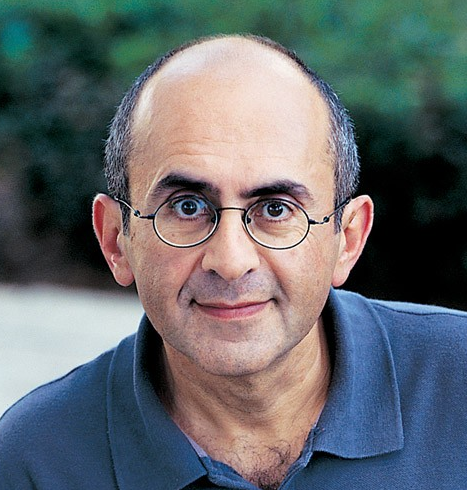
\includegraphics[width=4cm,height=5cm,keepaspectratio]{invited_img/falkovich}
		\end{center}
		\vspace{-20pt}
		\vspace{-10pt}
	\end{wrapfigure}
	Gregory Falkovich got PhD from Nuclear Physics Institute in Novosibirsk in 1984 and worked in Russian Academy of Science. In 1991 he left Russia for the Weizmann Institute of Science, where he works ever since, all the way from postdoctoral fellow to the department head. He is an author of a textbook "Fluid Mechanics (a short course for physicists)" based on twenty years of teaching the course on fluid mechanics. His work has been focused mostly on theory of turbulence on elementary level but connected as well to applications in geophysics, astrophysics and industry. He was awarded 4 awards of the Russian Academy of Science, one in Israel.
	
	\section*{Abstract} %\\
	The lecture is devoted to fundamental problems and modern applications of very viscous flows, from bacteria and microfluidics to quark-gluon plasma and electron flows in graphene. I start from explaining the nature of viscosity and then describe the purely geometrical world of inertia-less flows. I then describe new phenomena discovered in microfluidics and viscous electronics, from elastic turbulence to negative electric resistance.
	
         
    \vspace{.5cm}
    \newpage
    
